\section{ステップ1: 環境のセットアップ}

Dartではパワフルで生産的なツールが提供されています.その中で中心的な位置をしめるものがDart Editorです.Dart Editorは軽量なテキストエディタでDartのアプリケーションの実行,デバッグ,解析が行えます.エディタはDart SDKやDartium\footnote{Dart VMを搭載したChromium}と協調して動作をし,統一された体験を提供します.

\subsection{目標}

\begin{enumerate}
\item Dart Editorをインストール
\item Editorチームにフィードバックを送信
\item 時計のDartアプリケーションを実行
\item Dartiumについて学ぶ
\end{enumerate}

\subsection{ウォークスルー}

\subsubsection{Dart Editorをインストール}

タスク: GoogleIOの時と配布方式が異なるので,記述を変更

To get your environment set up, plug in the provided USB. Open the USB drive and find the \url{editor/} directory inside. Copy over the correct Dart Editor version for your OS/bit combination directory to your machine, and unzip it.

[Image]

Open up the newly unzipped \url{dart/} directory, and double click the executable:

\begin{itemize}
\item DartEditor.app (Mac)
\item DartEditor (Linux)
\item DartEditor.exe (Windows)
\end{itemize}

[Image]

Dart Editorを初めて起動すると,ようこそ画面が表示されます.

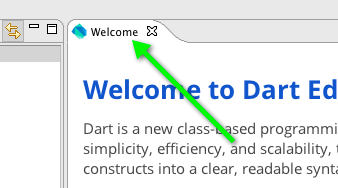
\includegraphics{step1/welcome.png}

\subsubsection{フィードバックを送るボタンを使う}

フィードバックをいただけるとDart Editorチームはとても感謝します.Dart Editorチームにあなたの考え(フィードバック)を知らせる最も簡単な方法はエディタのツールバーの右上にある''Send Feedback''と書かれたボタンを利用することです.

Send Feedbackボタンへマウスを移動しクリックします.

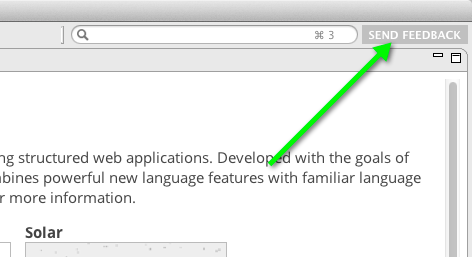
\includegraphics{step1/sendfeedback1.png}

Dart Editorのフィードバックダイアログを利用することで,エディタのチームに直接バグやリクエストを送信することができます.送信していただいた提案はバグレポートや機能リクエストとして登録させていただきます.\footnote{\url{http://dartbug.com}が私達のIssue Trackerです.}

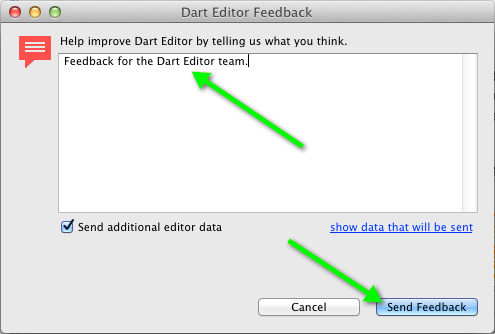
\includegraphics{step1/sendfeedback2.png}

\subsubsection{時計のサンプルを実行する}

(フィードバックウインドウが開いているときは,閉じてください.)

Dartのアプリケーションを実行してみましょう!

ようこそ画面からClock sampleをクリックします.これをクリックすることで,DartEditorにClock Sampleがコピーされ,新しいプロジェクトがセットアップされます.

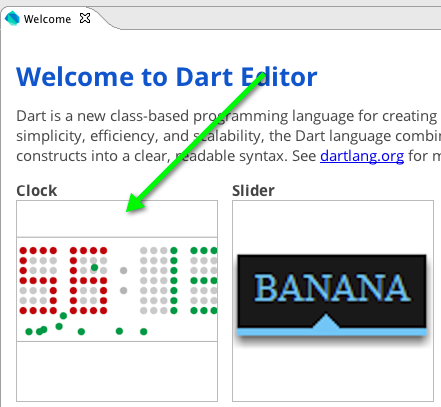
\includegraphics{step1/clocksample1.png}

ヒント: ようこそ画面が見つかりませんか? Toolsへ移動して,Welcome Pageをクリックすることで再度表示することができます.

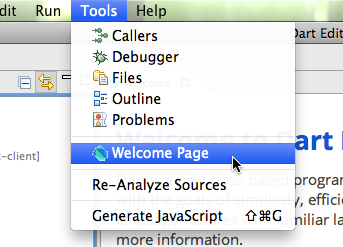
\includegraphics{step1/clocksample2.png}

ファイルビューではClock Sampleのすべてのファイルが表示されています.そこにはDartファイルはもちろん,アプリケーションをホストするHTMLファイル,また,すべてのイメージやCSSも同様に含まれています.clock.dartが''clock''ライブラリを定義しているDartファイルです.そして,そのファイルがこのサンプルのmain()関数を含んでいます.clock.dartファイルはエディタに自動的に開かれます.

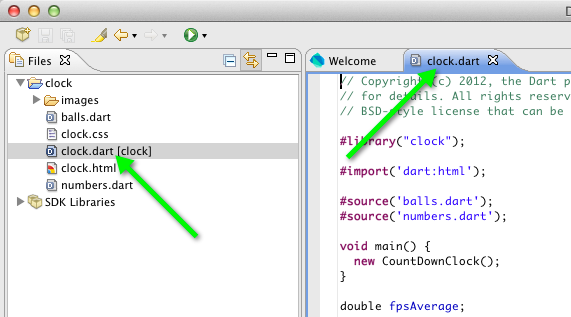
\includegraphics{step1/clocksample3.png}

clock.dartファイルが選択されて,ハイライトされていることを確認してください.DartエディタのRunボタンを押してください.このボタンを押すことでDartiumをロードし,アプリケーションが起動され,clock.htmlファイルをDartiumが開きます.

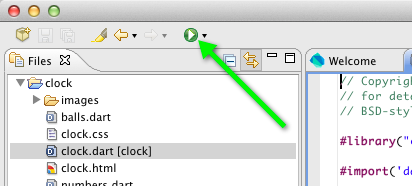
\includegraphics{step1/clocksample4.png}

Clock sampleアプリケーションがDartiumの中で動いています.おめでとうございます!初めてのDartアプリケーションが起動しました!

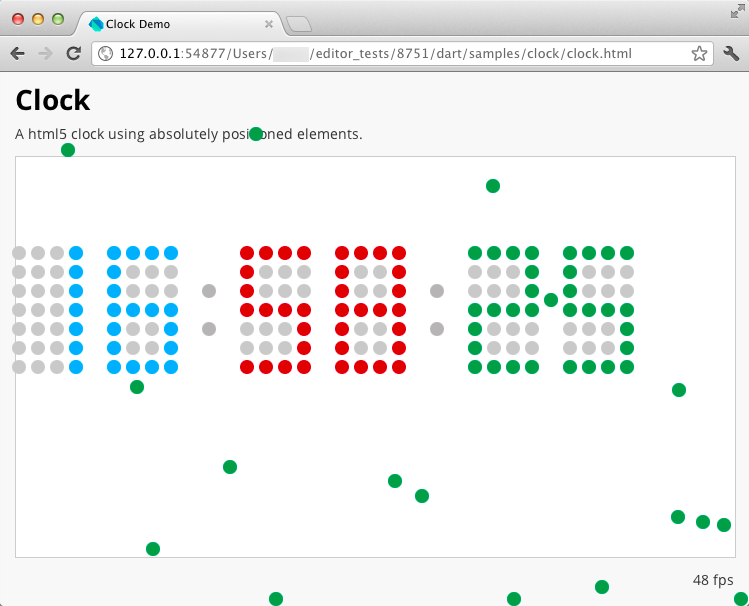
\includegraphics[width=13cm]{step1/clocksample5.png}

\subsubsection{Dartium}

Dartium is Chromium with an embedded Dart virtual machine (VM). Even though Dart compiles to JavaScript, you can speed up the "edit, reload" development cycle by running Dart apps directly in the browser.

To verify that Clock is running in Dartium, right-click in the browser and select Inspect Element.

[Image]

The Elements tab should be selected by default, and clock.dart should be listed as the script that is being run.

[Image]

\subsubsection{Debug with the Dart Editor}

With Dart running directly in Dartium, the editor has debugging support for Dart applications. Set a breakpoint by double clicking in the left hand gutter in Dart Editor on first call to setDigits() inside the updateTime() method in clock.dart, line 66. With the breakpoint set (you will see a little blue dot in the gutter), click the Run button again.

[Image]

Notice how the program stop, and the Debugger view opens in the Dart Editor. To continue the program without leaving the debugger, click the Resume button (the green arrow in the Debugger view). The updateTime() method is called every 1000ms, therefore the breakpoint will be hit again within a second.

[Image]

The Debugger view on the right hand side allows you to see which processes are running and what values are in scope at the breakpoint. Hover over the now field, the value will be displayed in a tooltip.

[Image]

To terminate the debugger, click on the red square in the Debugger view. This will also stop the application.

[Image]

\subsection{Advanced}

Load and launch the other samples.
In the Clock sample, try changing the ball velocity or the gravity. Start with lines 12 and 117 in balls.dart.
Set more breakpoints and inspect the values by opening up the variables.

[Image]
